\section{Background and Related Work}\label{sec:background}

\begin{figure*}[!ht]
    \centering
    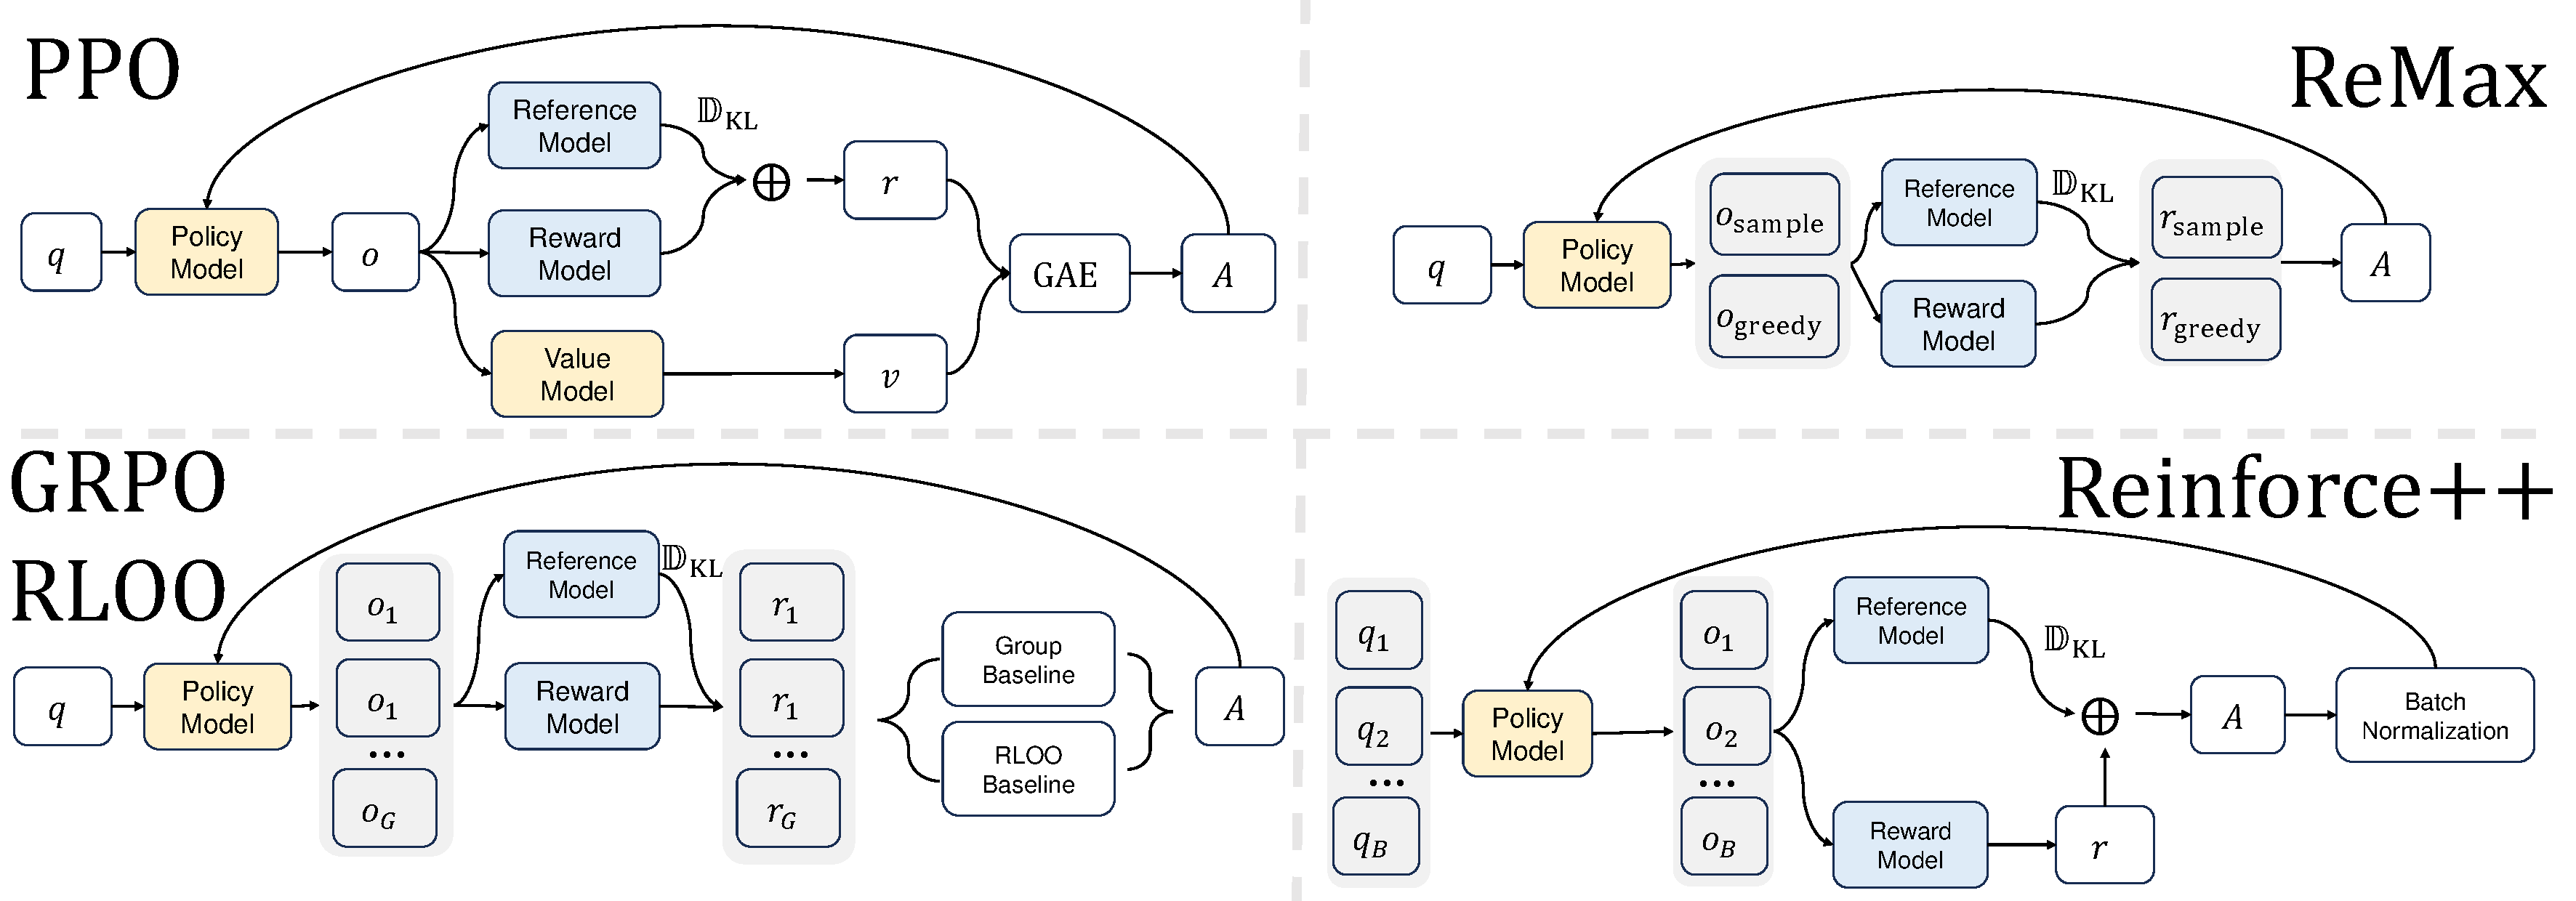
\includegraphics[width=0.85\textwidth]{imgs/re_2.pdf}
    \caption{The comparison of PPO, ReMax, GRPO, RLOO, and \ours. \ours, as shown in the figure, removes the critic model and uses global batch normalization. \varn uses group sampling, similar to GRPO/RLOO, but replaces the local group baseline with a group-mean subtraction followed by global batch normalization.}
    \label{fig:main}
\end{figure*}

\subsection{PPO and Critic-Free RLHF}
PPO optimizes LLMs by maximizing the following surrogate objective:

\begin{equation}\label{eq:ppo}
\begin{adjustbox}{max width=\linewidth}
$
\begin{aligned}
\mathcal{L}_{\text{PPO}}(\theta)
&= \mathbb{E}_{q \sim P(Q),\, o \sim \pi_{\theta_{\text{old}}}(O|q)} \Bigg[
    \frac{1}{|o|} \sum_{t=1}^{|o|}
    \min \Big(
        s_t(\theta) A_t, \\[-2pt]
&\quad \text{clip}(s_t(\theta),\, 1 - \epsilon,\, 1 + \epsilon) A_t
    \Big)
\Bigg]
\end{aligned}
$
\end{adjustbox}
\end{equation}

where $s_t(\theta) = \frac{\pi_{\theta}(o_t | q, o_{<t})}{\pi_{\theta_{\text{old}}}(o_t | q, o_{<t})}$ is the probability ratio. The advantage $A_t$ is typically calculated using Generalized Advantage Estimation~(GAE) \citep{schulman2015high}:
\begin{equation}
    A_{q, o_t} = \sum_{l=0}^{\infty} (\gamma \lambda)^l \delta_{t+l}
\end{equation}
where $\delta_{q, o_t} = r_t + \gamma V(o_{t+1}) - V(o_t)$ is the temporal difference error, and $V(\cdot)$ is the critic network.

Critic-free methods in \Cref{fig:main} remove the critic $V(\cdot)$ and compute the advantage $A_t$ directly from rewards.
\begin{itemize}[leftmargin=*]
    \item \textbf{ReMax} \citep{li2023remax} uses a greedy decoding response $\hat{o}$ as the baseline: $A_{q,o_t} = r(o) - r(\hat{o})$.
    \item \textbf{RLOO} \citep{2024Back} samples $k$ responses and uses the mean of others as the baseline: $A_{q,o_t^{(i)}} = r(o^{(i)}) - \frac{1}{k-1}\sum_{j \neq i} r(o^{(j)})$.
    \item \textbf{GRPO} \citep{shao2024deepseekmath} also samples $k$ responses but normalizes the advantage using the mean and standard deviation of the \textit{local group}:
\end{itemize}
\begin{equation}\label{eq:grpo}
A_{q,o_t^{(i)}} = \frac{r(o^{(i)}) - \text{mean}\bigl(\{r(o^{(j)})\}_{j=1}^{k}\bigr)}{\text{std}\bigl(\{r(o^{(j)})\}_{j=1}^{k}\bigr) + \epsilon}
\end{equation}

\subsection{The Problem with Local Normalization}
The core issue with methods like GRPO lies in \Cref{eq:grpo}. The usage of \textbf{prompt-level (local) normalization} is problematic for three reasons:
\begin{enumerate}
    \item \textbf{Theoretical Bias}: As formally proven in Appendix \Cref{appendix:proof_GRPO}, the estimator is biased. Therefore, the numerator (centered reward) and the denominator (local standard deviation $\text{std}(\cdot)$) are not independent. The denominator's value is correlated with the rewards in the small group, introducing a systematic error in the advantage estimate \citep{mai2025agent}.
    \item \textbf{Practical Instability}: In practice, the group size $k$ is small (e.g., 4 or 8). If all sampled responses for a prompt happen to get similar rewards, the local $\text{std}(\cdot)$ approaches zero, causing the advantage to explode. It results in high variance and unstable training.
    \item \textbf{Task Overfitting}: The policy is rewarded for being "better than other samples from the same prompt," not for being "globally good." It can lead to overfitting on simple prompts where it's easy to generate diverse rewards, while failing to improve on complex prompts.
\end{enumerate}